\documentclass{IEEEcsmag}
\usepackage{graphicx}
\usepackage{float}
\usepackage{hyperref}
\renewcommand{\figurename}{Slika}
\usepackage[colorlinks,urlcolor=blue,linkcolor=blue,citecolor=blue]{hyperref}
%\expandafter\def\expandafter\UrlBreaks\expandafter{\UrlBreaks\do\/\do\*\do\-%\do\~\do\'\do\"\do\-}
%\usepackage{upmath,color}



\jmonth{Siječanj}
\jname{FER}
\jtitle{Paralelna implementacija kartaške igre Blackjack}
\pubyear{2024}

\newtheorem{theorem}{Theorem}
\newtheorem{lemma}{Lemma}


\setcounter{secnumdepth}{0}

\begin{document}

\sptitle{Paralelizam i konkurentnost}

\title{Paralelna implementacije kartaške igre Blackjack}

\author{Voditelj projekta: Sebastian Medjaković}
\affil{Fakultet elektrotehnike i računarstva, Unska 3, Zagreb}

\author{Nika Šljubura}
\affil{Fakultet elektrotehnike i računarstva, Unska 3, Zagreb}

\author{Nikola Marić}
\affil{Fakultet elektrotehnike i računarstva, Unska 3, Zagreb}

\author{Domagoj Capar}
\affil{Fakultet elektrotehnike i računarstva, Unska 3, Zagreb}

\author{Tomislav Kožul}
\affil{Fakultet elektrotehnike i računarstva, Unska 3, Zagreb}

\markboth{PARALELIZAM I KONKURENTNOST}{PARALELIZAM I KONKURENTNOST}

\begin{abstract}\looseness-1U sklopu ovog projekta razvijena je aplikacija za igru kartaške igre „Blackjack“. Aplikacija je razvijena koristeći programski jezik Erlang i razvojni alat Rebar3. Erlang nudi podršku za paralelno izvođenje programskog koda, što omogućuje igračima (modul „player“) da istovremeno komuniciraju s djeliteljem karata (modul „dealer“) te da istovremeno zatraže karte, bez mogućnosti da dobiju istu kartu.
\end{abstract}

\maketitle

\section{Uvod}
\vspace{5mm}
Blackjack \cite{rules} je kartaška igra u kojoj igrači ne igraju međusobno, već svaki igrač igra protiv kuće (kockarnice). Kada se igra uživo s fizičkim kartama, svaki igrač ima svoj potez kada smije igrati, a ostatak vremena čeka da drugi igrači odigraju vlastite poteze. Slična implementacija koristi se u većini online\break kockarnica.

Ako su u igri četiri igrača, svaki od njih će tri četvrtine vremena provedenog igrajući čekati svoj red za igru. U sklopu ovog projekta htjeli smo razviti aplikaciju koja će znatno smanjiti vrijeme čekanja na potez igrača. Samim time, poboljšali bismo vremensku efikasnost igre, a posljedično i igračevo\break iskustvo.

Kako bismo ostvarili navedeno, razvili smo aplikaciju koja igračima dopušta simultano igranje, bez čekanja na red. Kada dealer započne igru, svi igrači dobivaju karte te imaju pravo odigrati poteze u isto vrijeme, čime smo efektivno vrijeme igranja povećali s jedne četvrtine na približno\break jedan.

\newpage

\section{Pravila igre Blackjack}
\vspace{5mm}
Prije donošenja odluke o tehnologiji za implementaciju igre Blackjack, nužno je detaljno razumjeti pravila i tijek igre, moguće poteze igrača, logiku djelitelja i ishode ovisno o vrijednostima karata u ruci, no za početak, osvrnimo se na osnovna pravila\break igre.

Špil za kartanje igre Blackjack sastoji se od nekoliko standardnih špilova od pedeset i dvije karte, bez karte „joker“. Od tih karata, karte od 2 do 10 nose vrijednost jednaku vlastitom broju, tako na primjer karta „3 srce“, nosi vrijednost 3. Karte „dečko“, „dama“ i „kralj“ nose vrijednost deset, dok situacija s kartom „as“ nije toliko jednostavna. Naime, početna vrijednost karte „as“ iznosi jedanaest – tada kažemo da je ruka „soft“. Ukoliko je zbroj vrijednost karata u ruci veći od dvadeset jedan i ruka sadrži kartu „as“, utoliko iznos njezine vrijednost više nije jedanaest, već jedan, čime ruka postaje\break „hard“.

Na početku igre, nakon što su igrači postavili svoje uloge, djelitelj dijeli po dvije karte svakom igraču i otkriva vrijednost jedne od svojih karata. Po primitku karata, svaki od igrača donosi jednu od dvije moguće odluke: zatražiti novu kartu od djelitelja (tzv. „hit“) ili nastaviti igrati s trenutnim kartama (tzv. „stand“). Ne postoji ograničenje koliko karata igrač može zatražiti od djelitelja, sve dok je zbroj vrijednosti karata u igračevoj ruci manji ili jednak dvadeset\break jedan. 

Ako je u igračevoj ruci po dobitku prve dvije karte jednak dvadeset jedan, igrač je ostvario „blackjack“ (termin po kojem je igra dobila ime), čime igrač automatski osvaja iznos jednak jedan i pol puta veći od uloga te je igra za njega gotova. Blackjack se postiže samo s dvije karte: „Asom“ i kartom vrijednosti deset. S druge strane, ako je zbroj karata u igračevoj ruci premaši  dvadeset jedan (tzv. „bust“), maksimalni zbroj vrijednosti je premašen, što označava gubitak uloga za igrača i kraj njegove\break igre. 

Nakon što su svi igrači, osim onih koji su ostvarili „blackjack“ ili „bust“, spremni za nastavak igre s trenutnim kartama („stand“), djelitelj igračima otkriva vrijednost svoje druge karte. Ako je zbroj vrijednosti karata u djeliteljevoj ruci manji od sedamnaest, tada djelitelj izvlači još jednu kartu. Ako je zbroj karata u djeliteljevoj ruci veći od dvadeset jedan („bust“), svaki od igrača koji su još u igri osvaja iznos dvostruko veći od njihovog uloga. Inače, samo igrači koji su nastavili igrati te čiji je zbroj vrijednosti karata u ruci veći od zbroja karata u djeliteljevoj ruci osvajaju iznos dvostruko veći od uloga, dok svi ostali aktivni igrači gube svoj\break ulog. 

Time je završena igra te nova igra započinje postavljanjem uloga od strane igrača. Pošto djelitelj predstavlja kuću (kockarnicu), on ne stavlja ulog. Djelitelj je na dobitku ako igrači\break gube.

U pravilima igre Blackjack pojavljuju se uloge djelitelja i igrača. Obije uloge bit će implementirane u zasebnim modulima. Raspodjelom funkcionalnosti u odvojene module omogućit ćemo bolju čitljivost, skalabilnost i olakšati ponovnu upotrebu komponenata\break igre. Dijagram tijeka igre Blackjack prikazan je na \textit{slici 1}.

% Then, where you want your figure:
\begin{figure*}[htbp]
\centering
\includegraphics[width=\textwidth]{flow-diagram.jpg}
\caption{Dijagram tijeka igre Blackjack u kojoj je na poslužitelja (djelitelja) spojen najmanje jedan klijent (igrač)}
\vspace{-5pt}
\end{figure*}

\section{Funkcionalnost djelitelja}
\label{sec:djelitelj}
\vspace{5mm}
Djeliteljeva glavna zadaća je raspodjela karata igračima. Iako se djeliteljev zadatak čini banalnim, dijeljenje karata i komunikacija s igračima omogućuju mu upravljanje tijekom igre. Budući da djelitelj ne sudjeluje direktno u igri, već se ponaša u skladu s igračevim zahtjevima i predefiniranim pravilima, u kontekstu aplikacije, ulogu djelitelja možemo dodijeliti\break poslužitelju (\textit{engl}. server).

Prije nego početka same igre, djeliteljev zadatak je promiješati karte, odnosno, ako pričamo o programskoj implementaciji djelitelja, generirati špil za igru. Djelitelj započinje igru kada svakom od igrača podijeli dvije karte te ih obavijesti o karti koju je sam\break izvukao.

Na zahtjev igrača za vrijeme njegova poteza, djelitelj istome dodjeljuje novu kartu iz špila, sve dok je zbroj vrijednosti karata u ruci igrača manji od dvadeset jedan. Kada su svi igrači spremni za nastavak igre („stand“, „bust“ ili „blackjack“), djelitelj igračima otkriva svoju drugu kartu te vuče nove karte sve dok je zbroj vrijednosti karata u njegovoj ruci manji od\break sedamnaest.

Kada je spomenuta suma vrijednosti premašena, djelitelj igrače obavještava o zbroju vrijednosti karata u ruci te nakon podjele osvojenih iznosa započinje novu igru. Također, ako broj karata u igračem špilu padne ispod određene vrijednosti, djelitelj promiješa preostale i već iskorištene karte, čime se igraći špil vraća u početno\break stanje.


\section{Funkcionalnost igrača}
\label{sec:igrac}
\vspace{5mm}
Ako djelitelju dodjeljujemo ulogu poslužitelja, u istom kontekstu igrač ima ulogu klijenta (engl. client). Klijent (računalo „igrač“) se spaja na poslužitelj (računalo „djelitelj“) čime započinje njihova komunikacija. Broj igrača koji sudjeluju u jednoj igri nije\break ograničen. 

Po ulasku u igru, igrač kroz korisničko sučelje unosi iznos ukupnih raspoloživih sredstava te na početku svake igre unosi svoj ulog za istu. Nakon što su mu dodijeljene karte, igrač bira želi li novu kartu ili želi nastaviti igrati s kartama koje trenutno ima u ruci. Igraču su na raspolaganju iste opcije po dodjeli svake nove karte, sve dok zbroj vrijednosti karata u njegovoj ruci ne premaši dvadeset jedan, kada o istome obavještava djelitelja i završava igru. S druge strane, ako je pri prvoj dodjeli karata ostvario Blackjack, odnosno dobio karte ukupne vrijednosti dvadeset jedan, odmah osvaja adekvatan iznos i završava\break igru. Također, igrač za vrijeme igre može promijeniti ulog (tzv. "stake").

Ako je igrač i dalje u igri, ishod se određuje po primitku ukupne vrijednosti djeliteljeve ruke. Ako je iznos ukupne vrijednosti karata u igračevoj ruci veći od onog u djeliteljevoj, igrač pobjeđuje i vrši se isplata. U suprotnom, igrač je\break izgubio.

Po završetku svake igre, igrač ponovo unosi svoj ulog i započinje nova\break igra. 

\newpage


\section{Paralelizacija igre Blackjack}
\vspace{5mm}
U tradicionalnoj igri s fizičkim kartama, protekne određeno vrijeme prije samog početka igre dok djelitelj svakom igraču podijeli dvije karte. Budući da je u aplikaciji nasumične karte moguće „izvući“ (generirati) i o istima obavijestiti igrača gotovo trenutno, taj vremenski period možemo zanemariti. Trenutnom dodjelom karata smo ubrzali tijek igre u odnosu na igru s fizičkim kartama. Radi vjerodostojnije usporedbe paralelnog i serijskog izvođenja igre, oba slučaja su promotrena u kontekstu\break aplikacije (trenutno generiranje karata).

Ako svaki igrač (osim prvog) mora čekati završetak poteza prethodnog igrača kako bi započeo vlastiti, radi se o \textbf{serijskom} izvođenju igre, čiji je dijagram tijeka prikazan\break na \textit{slici 2}. 

\begin{figure}[H]
\centerline{
\includegraphics[width=18.5pc]{serijsko-bijelo.png}}
\caption{Dijagram tijeka \textit{serijskog} izvođenja igre gdje je vrijeme trajanja poteza svakog igrača označeno s 'TRAJANJE POTEZA IGRAČA X', gdje 'X' označava redni broj igrača, a 'n' ukupni broj igrača}
\vspace*{-5pt}
\end{figure}

Kod serijskog izvođenja, ukupno vrijeme trajanja igre jednako je zbroju trajanja poteza svakog pojedinog igrača. Ukupno trajanje igre računa se prema formuli \textit{(1)}, gdje $T_{ukupno}$ označava ukupno trajanje igre, $T_x$ vrijeme trajanja poteza igrača s rednim brojem $x$, a $n$ ukupan broj igrača.

\begin{equation}
T_{ukupno} = \sum_{x=1}^{n} T_x
\end{equation}



S druge strane, ako svi igrači započinju vlastiti potez u isto vrijeme, radi se o \textbf{paralelnom} izvođenju igre, čiji je dijagram tijeka prikazan\break na \textit{slici 3}.

\begin{figure}[H]
\centerline{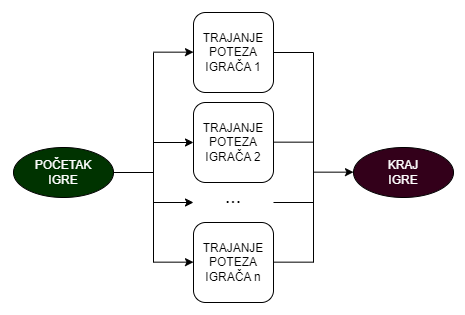
\includegraphics[width=18.5pc]{paralelnog-bijelo.png}}
\caption{Dijagram tijeka \textit{paralelnog} izvođenja igre gdje je vrijeme trajanja poteza svakog igrača označeno s 'TRAJANJE POTEZA IGRAČA X', gdje 'X' označava redni broj igrača, a 'n' ukupni broj igrača}
\vspace*{-5pt}
\end{figure}

Kod paralelnog izvođenja, ukupno vrijeme trajanja igre jednako je vremenu trajanja najduljeg poteza među igračima. Ukupno trajanje igre računa se prema formuli \textit{(2)}, gdje $T_{ukupno}$ označava ukupno trajanje igre, $T_x$ vrijeme trajanja poteza igrača s rednim brojem $x$, a $n$ ukupan broj igrača.

\begin{equation}
T_{ukupno} = \max{(T_1, T_2, ... , T_n)}
\end{equation}



Kako bismo odredili točan omjer efektivnog vremena provedenog igrajući Blackjack, pretpostavit ćemo da su vremena trajanja poteza svih igrača međusobno jednaka i to vrijeme označit ćemo s $T_{potez}$, a ukupan broj igrača označit ćemo s $n$. Pod pretpostavkom da je vrijeme ukupnog trajanja igre \textbf{kraće u slučaju paralelnog izvođenja u odnosu na serijsko}, rezultat omjera ukupnog trajanja serijskog (označenog kao $T_{serijsko}$) i paralelnog (označenog kao $T_{paralelno}$) izvođenja označit će višestrukost ubrzanja paralelizacijom igre. Spomenuti omjer prikazan je u funkciji \textit{(3)}.

\begin{equation}
\begin{split}
\frac{T_{serijsko}}{T_{paralelno}} &= \frac{\sum_{x=1}^{n} T_{potez}}{\max{(T_{potez}, T_{potez}, ... , T_{potez})}} \\
&= \frac{n * T_{potez}}{T_{potez}} \\
&= n
\end{split}
\end{equation}

Paralelnim izvođenjem igre Blackjack trajanje igre skratili smo \textbf{približno \textit{n} puta}, gdje je $n$ ukupan broj igrača.
\newpage

\section{Problem paralelnog izvođenja}
\vspace{5mm}
U programskoj implementaciji igre Blackjack, želimo igraći špil simulirati što vjerodostojnije fizičkom špilu u tradicionalnoj igri, stoga, nakon izvlačenja karte, istu želimo ukloniti iz špila. Budući da su svi igrači na potezu u isto vrijeme, postoji mogućnost da dva ili više igrača kartu zatraže istovremeno. Djelitelj istu fizičku kartu ne može dodijeliti dva igrača, stoga taj scenarij moramo spriječiti. Budući da smo igru odlučili implementirati paralelno, igrače možemo gledati kao \textbf{zasebne dretve}. Špil karata je zajednički resurs svim igračima, pa je potrebno onemogućiti višestruki istovremeni pristup istome, što je zahtjev koji će igrati ključnu ulogu pri odabiru programske potpore za razvoj igre.

\section{Programska implementacija igre Blackjack}
\vspace{5mm}
Glavni uvjet pri odabiru programskog jezika za implementaciju igre Blackjack je da igraći špil bude dostupan u svakom trenutku, uz onemogućavanje višestrukog istovremenog pristupa resursu. Programski jezik koji zadovoljava ovaj uvjet visoke dostupnosti je Erlang \cite{erlang}. Dodatno, korišten je alat Rebar3 \cite{rebar3}, koji je pružio funkcionalnosti potrebne za lakše pokretanje i\break izgradnju modula.

Iako je uvjet visoke dostupnosti vrlo važan, nije jedini potreban za programsku implementaciju igre. Kako bi igra uopće mogla biti pokrenuta, potrebno je omogućiti komunikaciju djelitelja (poslužitelja) i igrača (klijenata). Za to smo koristili Erlangov \textit{gen\_server} modul ponašanja, koji pruža funkcionalnosti generičkog \textbf{klijent-poslužitelj}\break odnosa \cite{gen_server}.

Za komunikaciju djelitelja i igrača korištene su procedure za obradu zahtjeva \textit{'call'} (omogućuje \textbf{sinkronu} komunikaciju) i \textit{'cast'} (omogućuje \textbf{asinkronu} komunikaciju). Obije procedure služe za poziv funkcija ili obradu zahtjeva unutar istog modula (na primjer, kada poslužitelj šalje zahtjev koji se obrađuje unutar istog poslužitelja, ili analogno za klijenta) te između različitih, međusobno povezanih, modula (na primjer, kada funkcija s klijenta poziva funkciju na poslužitelju, ili obrnuto). Prilikom korištenja \textit{sinkrone} komunikacije, program unutar modula nastavlja s izvršavanjem nakon završetka obrade zahtjeva ili izvođenja funkcije. Nasuprot tome, kod \textit{asinkrone} komunikacije program odmah nastavlja s izvršavanjem, ne čekajući završetak\break obrade.

Stanje modula (\textit{engl}. \textbf{state}) omogućuje je pohranu podataka relevantnih za upravljanje tokom igre. Tako poslužitelj čuva špil igraćih karata, ažurirajući ga po izvlačenjem svake karte, kao i zbroj vrijednosti karata u vlastitoj ruci i broj igrača koji više ne sudjeluju u igri. Broj neaktivnih igrača koristi za računanje kako bi znao jesu li svi preostali igrači spremni. Igrač je također morao ažurirati zbroj vrijednosti karata u ruci te pratiti balans i uloge. Kada igrač želi zatražiti novu kartu, ne može špilu pristupiti izravno, već to čini slanjem zahtjeva poslužitelju. U Erlangu nije moguć paralelan pristup podacima spremljenima u \textit{stanje}, već se pristup i obrada istih obrađuje sekvencijalno. Time je onemogućen istovremeni pristup špilu od strane više igrača, što rješava ključni problem paralelne implementacije igre Blackjack. Ovaj pristup nije ograničen isključivo na implementaciju igre Blackjack; sličan pristup može se primijeniti u širokom spektru domena s problemima zajedničkog\break pristupa resursima. 

Implementacijom ponašanja navedenih u poglavlju \hyperref[sec:djelitelj]{\textit{Funkcionalnosti djelitelja}} u modul servera te onih navedenih u \hyperref[sec:igrac]{\textit{Funkcionalnosti igrača}} u modul klijenta i njihovim povezivanjem, uspjeli smo ispuniti sve zahtjeve potrebne za provođenje igre Blackjack.


\section{Simulacija igre Blackjack}
\vspace{5mm}
Na samome kraju, prije zaključka, proveli smo nekoliko simulacija igre Blackjack s različitim ishodima.

Budući da je djelitelj automatiziran, na konzoli djelitelja nije bilo ispisa. Sve djeliteljeve poruke bile poslane igračima te prikazane na njihovim korisničkim sučeljima, stoga su na slikama prikazane korisničke konzole.
Kada igrač pokrene igru, pokušava se kao klijent spojiti na poslužitelja, odnosno djelitelja. Nakon uspješnog spajanja, igrač treba unijeti svoj balans te ulog za prvu igru. Opisani proces pokretanja igre prikazan je na \textit{slici 4}.

\begin{figure}[H]
\centerline{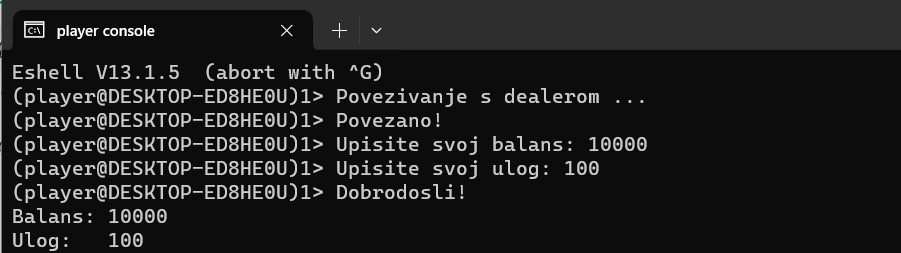
\includegraphics[width=18.5pc]{1.jpeg}}
\caption{Povezivanje igrača s poslužiteljem (djeliteljem) i početak igre}
\vspace*{-5pt}
\end{figure}

Budući da se igra provodi naredbama u konzoli, implementirana je naredba „help“, koja korisniku ispisuje sve implementirane naredbe i njihova značenja. Ispis na konzoli nakon poziva naredbe „help“ prikazan je na \textit{slici 5}. Također, nakon naredbe „help“, pozvana je naredba „stake“, čime je igraču omogućena promjena uloga.

\begin{figure}[H]
\centerline{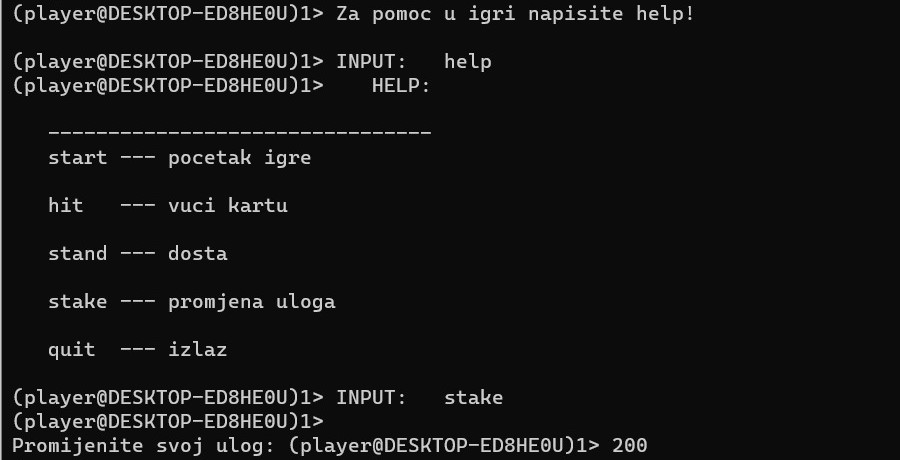
\includegraphics[width=18.5pc]{2.jpeg}}
\caption{Poziv naredbe \textit{"help"} te promjena uloga}
\vspace*{-5pt}
\end{figure}

Prvi prikazani ishod igre je gubitak igrača, preciznije gubitak premašivanjem maksimalne dozvoljene vrijednosti zbroja sume karata u igračevoj ruci. Na \textit{slici 6}, prikazan je slučaj kada je zbroj vrijednosti karata u igračevoj ruci bio jednak 24. Budući da je maksimalna dozvoljena vrijednost ruke jednaka 21, igrač je ostvario „bust“, što je i prikazano na konzoli. Također, vidimo da se balans igrača smanjio za iznos jednak ulogu.

\begin{figure}[H]
\centerline{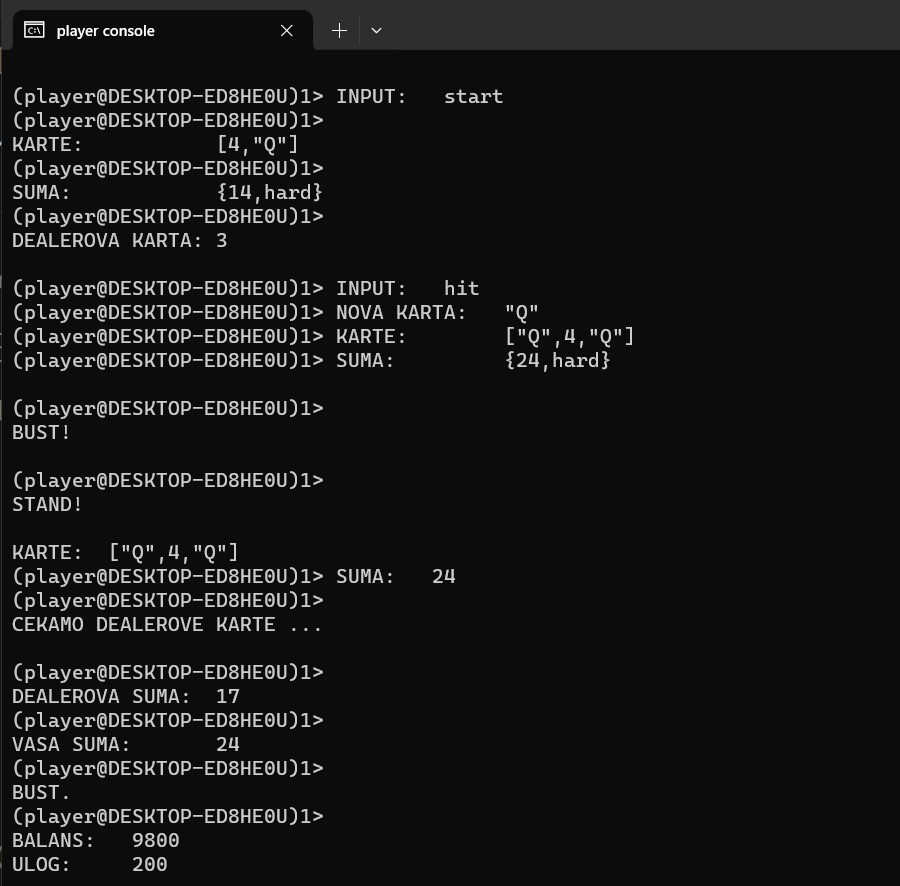
\includegraphics[width=18.5pc]{3.jpeg}}
\caption{Simulacija igre i gubitak igrača}
\vspace*{-5pt}
\end{figure}

Na \textit{slici 7}, prikazana je simulacija igre u kojoj je na kraju suma vrijednosti karata u igračevoj ruci bila veća od djeliteljeve sume, čime je igrač pobijedio u igri i osvojio iznos jednak ulogu.

\begin{figure}[H]
\centerline{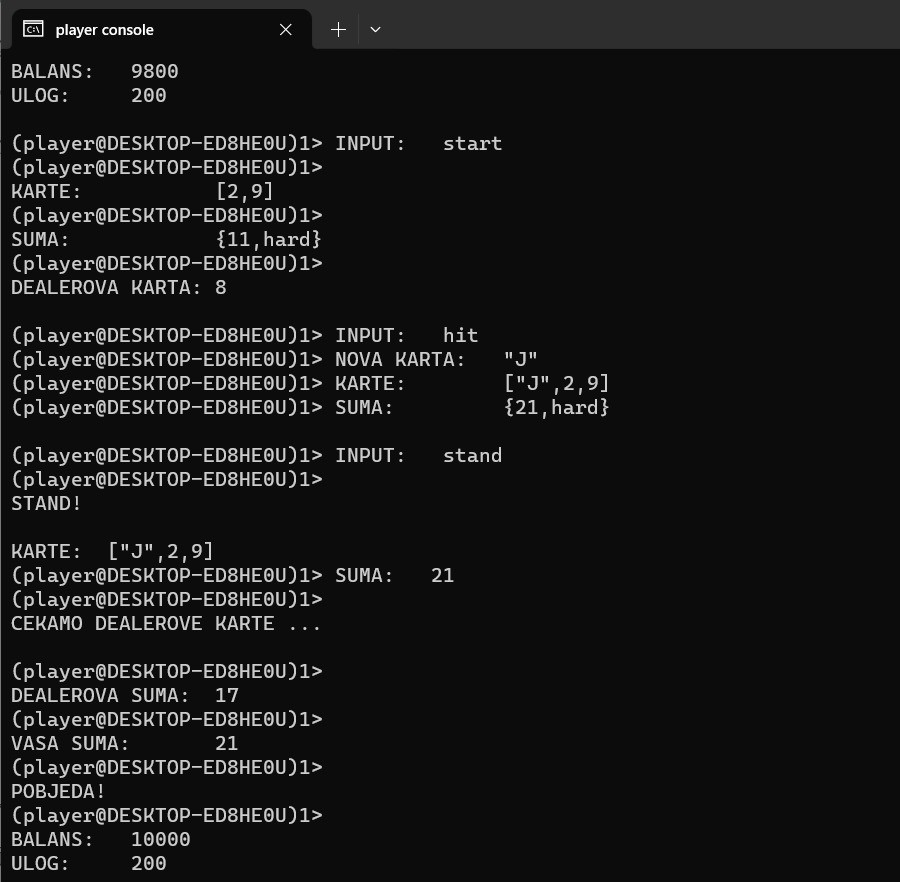
\includegraphics[width=18.5pc]{4.jpeg}}
\caption{Simulacija igre i pobjeda igrača}
\vspace*{-5pt}
\end{figure}




\section{Zaključak}
\vspace{5mm}
Koristeći programski jezik Erlang te funkcionalnosti gen\_server modula, implementirali smo aplikaciju koja igračima omogućuje igranje kartaške igre Blackjack. U igri postoje dvije uloge: djelitelj, koji je implementiran kao modul poslužitelj, i igrač, koji ima ulogu klijenta.  Za razliku od tradicionalne igre s fizičkim kartama, igrači ne moraju čekati red na potez, već svi igrači igraju svoj potez istovremeno, čime je trajanje jedne igre ubrzano približno $n$ puta, gdje je $n$ broj igrača koji sudjeluju\break u igri.

Htjeli smo da simulacija igre bude što vjerodostojnija tradicionalnoj igri, zbog čega smo napravili zajednički špil karata koji je univerzalan za sve igrače. Budući da je igraći špil pohranjen u djeliteljevom stanju (\textit{engl}. state), onemogućen je višestruki istovremeni pristup špilu. 


\def\refname{Literatura}

\begin{thebibliography}{1}

\bibitem{rules}
\url{www.en.wikipedia.org/wiki/Blackjack}, pristupljeno 20. siječnja 2024.

\bibitem{erlang}
\url{www.erlang.org}, pristupljeno 21. siječnja 2024.

\bibitem{gen_server}
\url{www.erlang.org/doc/man/gen_server.html}, pristupljeno 21. siječnja 2024.

\bibitem{rebar3}
\url{www.rebar3.org/}, pristupljeno 21. siječnja 2024.

\end{thebibliography}\vspace*{-8pt}

\end{document}